\vspace{0.2cm}
\noindent
这就把张量直接与\emph{多元多项式}联系了起来。上面的标量映射
\[
f(\xb^{(1)},\dots,\xb^{(N)})=\sum_{i_1,\dots,i_N}\Tt_{i_1\cdots i_N}\,\xb^{(1)}_{i_1}\cdots \xb^{(N)}_{i_N},
\]
是关于各向量分量的多项式，并且是\emph{多重线性}的：每个变量出现的次数至多为一（就每一组变量 $\xb^{(k)}$ 而言如此）。在一个重要的特殊情形中，所有输入都是\emph{同一个}向量 $\xb\in\RR^{d}$，而 $\Tt\in\RR^{d\times\cdots\times d}$ 有 $N$ 个模，此时收缩
\[
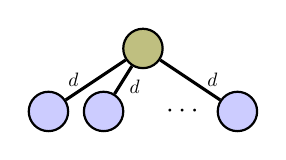
\begin{tikzpicture}[baseline=2ex]
    \tikzset{tensor/.style = {minimum size = 0.5cm,shape = circle,thick,draw=black,inner sep = 0pt},
             edge/.style   = {thick,line width=.4mm},
             every loop/.style={}}
    \def\x{0}\def\y{0}

    \node[tensor,fill=green!50!red!50!white] (T) at (\x,\y+0.8){$\Tt$};

    \node[tensor,fill=blue!20!white] (a) at (\x-1.2,\y){$\xb$};
    \node[tensor,fill=blue!20!white] (b) at (\x-0.5,\y){$\xb$};
    \node[draw=none] (dots) at (\x+0.5,\y){$\cdots$};
    \node[tensor,fill=blue!20!white] (z) at (\x+1.2,\y){$\xb$};

    \draw[edge] (T) -- (a) node [midway,left]{\scalebox{0.7}{\dimcolor{$d\ $}}};
    \draw[edge] (T) -- (b) node [near end,right]{\scalebox{0.7}{\dimcolor{$d$}}};
    \draw[edge] (T) -- (z) node [midway,right]{\scalebox{0.7}{\dimcolor{$\ d$}}};
\end{tikzpicture}
= \Tt \ttm{1}\xb \ttm{2}\xb \cdots \ttm{N}\xb
=
\sum_{i_1,\dots,i_N}\Tt_{i_1\cdots i_N}\,\xb_{i_1}\cdots \xb_{i_N} \in \RR.
\]
是一个 $N$ 次\emph{齐次}多元多项式（每个单项式的总次数恰为 $N$）。张量的分量恰好是这一多项式在单项式基 $(\xb_{i_1}\cdots \xb_{i_N})_{i_1,\cdots,i_N}$ 下的系数。

反之，若把 $(N+1)$ 阶张量 $\Tt\in\RR^{ d\times\cdots\times d \times p}$ 与 $N$ 份 $\xb\in\RR^d$ 收缩，并让最后一条腿保持自由，就得到一个向量值的齐次多项式映射 $\RR^d\to\RR^m$：
\[
p(\xb) = \Tt \ttm{1}\xb \ttm{2}\xb\cdots \ttm{N}\xb \in\RR^{p}.
\]

\vspace{0.2cm}
\noindent
最后，\emph{非齐次}多项式可以用一个小技巧得到：\emph{在输入向量末尾添上一个常数 $1$}。设 $\xb\in\RR^d$，并定义增广向量 $\tilde{\xb} =\begin{bmatrix}\xb\\1\end{bmatrix}\in\RR^{d+1}$。若 $\widetilde{\Tt}\in\RR^{(d+1)\times\cdots\times(d+1)}$ 是一个 $N$ 阶张量，则
\[
\tilde{p}(\xb)
:=
\widetilde{\Tt} \ttm{1}\tilde{\xb}\ttm{2}\tilde{\xb}\cdots\ttm{N}\tilde{\xb},
\]
是 $\xb$ 的不超过 $N$ 次的多项式（某些因子会取到最后一个坐标，也就是常数 $1$，从而降低相应单项式的次数）。换句话说，增广变量 $(x_1,\dots,x_d,1)$ 的一个齐次张量多项式，就紧凑地表示了 $(x_1,\dots,x_d)$ 的一般多元多项式。这一观点在实践中尤为有用：只需给每个模添加一个额外的维度并把它固定为 $1$，就能用与齐次情形相同的收缩机制来处理偏置项与低次交互项。  
